\documentclass[letterpaper, 12pt]{article}
\usepackage[letterpaper, top=2.5cm, bottom=2.5cm, left=3cm, right=3cm]{geometry} %margenes
\usepackage[utf8]{inputenc} %manejo de caracteres especiales
\usepackage[spanish]{babel} %manejo de encabezados de inglés a español
\usepackage{fancyhdr} %formato de los encabezados de página
\usepackage{ragged2e} %alineado real justficado
\usepackage{graphicx} %manejo de imagenes
\usepackage{amsmath} %manejo de notación matemática
\usepackage{mathtools} %manejo de notación matemática
\usepackage{blindtext} %texto de relleno
\usepackage{cancel} %permite la simbolización de cancelación de terminos
\usepackage{enumitem}[shortlabels] %listas con letras
\usepackage{amssymb} %manejo de simbolog►1a matematica
\usepackage[titles]{tocloft} %manejo de elementos para el índice
\usepackage{float} %manejo de centrado para figuras
\usepackage{hyperref} %manejo d hipervínculos
\hypersetup{
    colorlinks=true,      
    urlcolor=blue,
    linkcolor=blue
}
\pagestyle{fancy}
\fancyhf{}
\rfoot{\thepage}


\begin{document}
    
    %PORTADA
    \begin{titlepage}
        \begin{figure}[ht]
            \centering
            
\includegraphics[width=15cm]{logosITT.png}
        \end{figure}
        \centering
        {\scshape\LARGE Tecnológico Nacional de México\\Instituto Tecnológico de Tijuana\par}
        \vspace{1cm}
        {\scshape\Large Cálculo Diferencial\par}
        \vspace{1cm}
        {\scshape\Large Unidad 1\par}
        \vspace{1.5cm}
        {\huge\bfseries Números Reales\par}
        \vfill
        Asesor: \par
        C. Abraham Jhared Flores Azcona
        
        \vfill

        {\large \emph{``If it's close enough, it's good enough.''}}


    \end{titlepage}

    \newpage
        \pagestyle{empty}
        \tableofcontents
        \listoffigures

        \newpage
        \pagestyle{fancy}
        \lhead{\textbf{Unidad 1: Números Reales}}
        \section{Los números reales}
        Sin acomplejar tanto, los números reales \emph{son el conjunto que incluye a los numeros enteros, racionales e irracionales} donde las operaciones básicas funcionan; su símbolo es: \(\mathbb{R}\). La ejemplificación del conjunto es la siguiente:
        \begin{figure}[H]
            \centering
            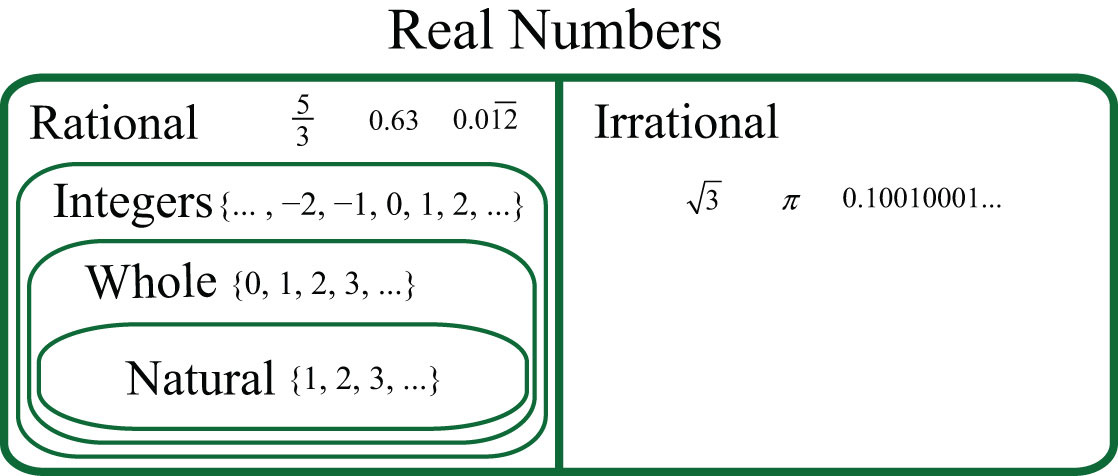
\includegraphics[width=10cm]{R.jpg}
            \caption{Diagrama de Venn de \(\mathbb{R}\).}
            \label{fig:R}
        \end{figure}
        Esto nos permite tener un mayor grado de libertad al momento de hacer cálculos.
        \section{Axiomas de los números reales}
        En otras palabras las reglas y propiedades que \(\mathbb{R}\) soporta. Algunas (si no es que todas) las hemos empleado de manera intuitiva sin saber sus nombres formales.
        \begin{figure}[H]
            \[\begin{matrix}
                \text{Identidad:}&a=a\\
                \text{Reciprocidad:}&\text{Si }a=b \text{ entonces } b=a\\
                \text{Transitividad:}&\text{Si }a=c \text{ y }b=c \text{ entonces }a=c\\
                \text{Uniformidad en la suma:}&\text{Si }a=b \text{ y }c=d \text{ entonces }a+c=b+d\\
                \text{Conmutatividad en la suma:}&a+b=b+a\\
                \text{Asociatividad en la suma:}&(a+b)+c=a+(b+c)\\
                \text{Módulo de la suma:}&a+0=0+a=a\\
                \text{Inverso aditivo:}&a+(-a)=0\\
                \text{Uniformidad en la multiplicación:}&\text{Si }a=b \text{ y }c=d \text{ entonces }ac=bd\\
                \text{Conmitatividad en la multiplicación}&ab=ba\\
                \text{Asociatividad en la Multiplicación}&(ab)c=a(bc)\\
                \text{Módulo del producto}&1\times a=a\times 1=a\\
                \text{Inverso mutiplicativo}&\forall a\neq 0,\, a\times \frac{1}{a}=1\\
            \end{matrix}\]
            \caption{Axiomas de \(\mathbb{R}\).}
            \label{fig:axiomasR}
        \end{figure}
        De estos se derivan las operaciones básicas. Las cuales según el acronimo \textbf{PEMDAS} son las siguientes:
        \begin{figure}[H]
            \[\begin{matrix}
                \text{P}&\text{Paréntesis}&(a)\\
                \text{E}&\text{Exponentes}&a^b\\
                \text{M}&\text{Multiplicación}&a\times b\\
                \text{D}&\text{División}&a/b\\
                \text{A}&\text{Adición (Suma)}&a+b\\
                \text{S}&\text{Substracción (Resta)}&a-b
            \end{matrix}\]
            \caption{Significado y ejemplos de PEMDAS.}
            \label{fig:PEMDAS}
        \end{figure}
        Son muchas propiedades, pero NO ES NECESARIO MEMORIZARLAS, como se ha planteado, el tener la noción (conocer que són pues) es mas que suficiente para avanzar en matemáticas de nivel superior.
        \section{Intervalos y su representación gráfica}
        Lo más importante que tenemos que tener en cuenta, es que debido a que \(\mathbb{R}\) contiene a los demás números, al representarlos en la linea recta; de un valor dado a otro (por ejemplo: de 1 a 2) existen \emph{una infinidad de valores entre ellos}.
        Es por eso que al graficar funciones con dominio en \(\mathbb{R}\) nos muestra un trazo bastante uniforme y continuo, en comparación con \(\mathbb{N}\) (números numeros) que, como se muestra en la siguiente imágen, quedaria un trazo ``moteado'' o solamente puntos sin unír en la función.
        \begin{figure}[H]
            \centering
            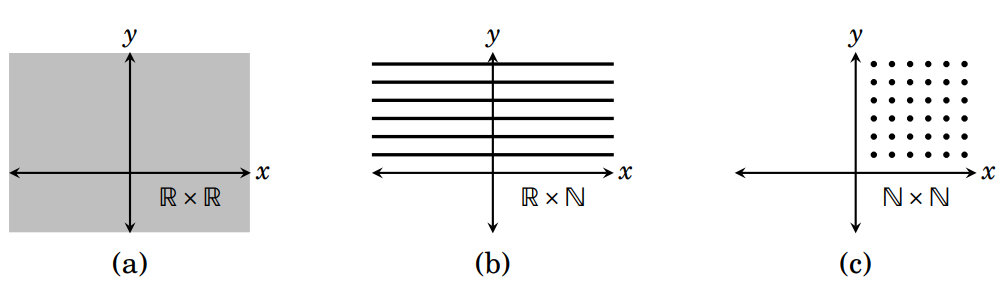
\includegraphics[width=10cm]{nvsr.PNG}
            \caption{Diferencia gráfica de dominios como producto cruz de \(\mathbb{N}\) y \(\mathbb{R}\).}
            \label{fig:nvsr}
        \end{figure}
        \section{Valor absoluto y sus propiedades}
        Simple y sencillamente, es \emph{el valor numérico sin tener en cuenta su signo}. En \(\mathbb{R}\) se define de la sig. manera:
        \begin{figure}[H]
            \[\begin{matrix}
                |a|&=&a\,\text{ si }a\geq 0\\
                |a|&=&-a\,\text{ si }a<0
            \end{matrix}\]
            \caption{Definición del valor absoluto.}
            \label{fig:abs}
        \end{figure}
        Es importante tener en cuenta que esta función \emph{es continua}. Otras equivalencias y propiedades son las siguientes:
        \begin{figure}[H]
            \[\begin{matrix}
            \text{No Negatividad}&|a|\geq 0\\
            \text{Definición positiva}&|a|=0\leftrightarrow a=0\\
            \text{Propiedad multiplicativa}&|ab|=|a||b|\\
            \text{Propiedad aditiva}&|a+b|\leq|a|+|b|\\
            \text{Simetría}&|-a|=|a|\\
            \text{Preservación de la división}&\left|\frac{a}{b}\right|=\frac{|a|}{|b|},\,\forall b\neq 0
            \end{matrix}\]
            \caption{Equivalencias del valor absoluto.}
            \label{fig:defextraabs}
        \end{figure}
        Otras inecuaciónes útiles para la resolución de desigualdades son las siguientes:
        \begin{figure}[H]
            \[\begin{matrix}
            |a|\leq b&\leftrightarrow&-b\leq a\leq b\\
            b\leq |a|&\leftrightarrow&a\leq-b \vee b\leq a\\
            |a-b|&\leq&|a-c|+|c-b|\\
            |a-b|&\geq&||a|-|b||
            \end{matrix}\]
            \caption{Equivalencias en forma de desigualdades del valor absoluto.}
            \label{fig:eqdesabs}
        \end{figure}
        Un ejemplo de ello es lo siguiente:
        \\\newline \textbf{Resolver la sig, inecuación:}
        \[|x-3|\leq 9\]
        1. Identificar la equivalencia parecida a la expresión:
        \[|x-3|\leq 9\sim|a|\leq b\]
        2. Identificar las variables para aplicar la equivalencia:
        \[a=x-3,\, b=9\]
        3. Sustituir en la equivalencia identificada:
        \[\begin{matrix}
            |a|\leq b&=&-b\leq a \leq b\therefore\\
                \therefore&=&-9\leq x-3\leq 9\\
        \end{matrix}\]
        4. Resolver para \(x\):
        \[\begin{matrix}
            -9\leq x-3\leq 9\\
            -9+3\leq x-3-3\leq 9+3\\
            -6\leq x\leq 12
        \end{matrix}\]
        \section{Propiedades de las desigualdades}
        Simple y sencillamente, la desigualdad es una expresión que indica ue una cantidad es mayor o menor que otra. Sus propiedades son las siguientes:
        \\\newline
        \textbf{Si a los dos miembros de una desigualdad se suma o resta una misma cantidad, el signo de la desigualdad no varía.}
        \[a+c>b+c \,\text{ y }\, a-c>b-c\]
        \textbf{Un término cualquiera de una desigualdad se puede pasar de un miembro a otr cambiándole el signo.}
        \[a>b+c\rightarrow a-c>b\]
        \textbf{Si los dos miembros de una desigualdad se multiplican o dividen por una misma cantidad positiva, el signo de la desigualdad no varía.}
        \[ac>bc\, \text{ y }\,\frac{a}{c}>\frac{b}{c}\]
        \textbf{Si los dos miembros deuna desigualdad se multiplican o dividen por una misma cantidad negativa, el signo de la desigualdad varía.}
        \[-ac<-bc\, \text{ y }\,-\frac{a}{c}<-\frac{b}{c}\]
        \textbf{Si se cambia el signo a todos los téerminos, o sea a los dos miembros de una desigualdad, el signo de la desigualdad varía.}
        \[-1(a-b>-c)=b-a<c\]
        \textbf{Si se cambia el orden de los miebros, la desigualdad cambia de signo.}
        \[\text{Si }a>b \text{ es evidente que }b>a\]
        \textbf{Si se invierten los dos miembros, la desigualdad cambia de signo.}
        \[\text{Si }a>b \text{ es evidente que }\frac{1}{a}<\frac{1}{b}\]
        \textbf{Si los miembros de una desigualdad son positivos y se elevan a una misma potencia positiva, el signo de la desigualdad no cambia.}
        \[(5)^2>(3)^2\rightarrow 25>9\]
        \textbf{Si los dos miembros son negativos y se elevan a una misma potencia par positiva, el signo de la desigualdad cambia.}
        \[(-3)^2>(-5)^2\rightarrow 9<25\]
        \textbf{Si los dos miembros de una desigualdad son positivos y se les extrae una misma raíz positiva, el signo de la desigualdad no cambia }
        \[\text{Si }a,b,n \text{ son positivos, tenemos }\sqrt[n]{a}>\sqrt[n]{b}\]
        \textbf{Si dos o más desigualdades del mismo signo se suman o multiplican miembro a miembro, resulta una desigualdad del mismo signo.}
        \[\text{Si }a>b, c>d \text{ son positivos, tenemos }a+c>b+d, ac>bd\]
        \section{Resolución de desigualdades de primer y segundo grado con una incógnita}
        Se conocen tambien como inecuaciones o desigualdades de condición. Mecanicamente es similar a resolver las igualdades que se han manejado anteriormente. 
        Ejemplos encontrados en las diapositivas de Miro
        \section{Resolución de desigualdades que incluyen valor absoluto}
        Ejemplos encontrados en las diapositivas de Miro.
        \section*{Hipervínculos de material complementario:}
        El acceso es CON CORREO INSTITUCIONAL.
        \begin{itemize}
            \item \href{https://docs.google.com/document/d/1mhFr7S5rJ7TwR297Kd6l8b6NPvYkUAlpWIxuz4VKV2w/edit?usp=sharing}{\textbf{Pizarras Online de Miro (compendio de los enlaces).}}
            \item \href{https://drive.google.com/drive/folders/1yL1gAIbVpgKB3h8498KFNE7NDZjoxIWa?usp=sharing}{\textbf{Carpeta de los Documentos PDF.}}
            \item \href{https://drive.google.com/drive/folders/1TPtNSe4ErSgaBLw2kgYDQadyXqvh6AYC?usp=sharing}{\textbf{Grabaciones de las asesorías y demás.}}
        \end{itemize}
\end{document}